
\section{backup slides}
\begin{frame}{backup slides}
\end{frame}

\subsection{data flow limit}
\usetikzlibrary{shapes,fit,arrows.meta,chains}

\begin{frame}[fragile,label=dfLimit]{data flow model and limits (1)}
    \begin{tikzpicture}
        \tikzset{
            var/.style={draw,rectangle,fill=blue!30},
            op/.style={draw,ellipse,fill=yellow!40},
            node distance=4mm,
        }
        \begin{scope}[
                start chain=going below,
                every join/.style={thick,-Latex},
                every node/.style={on chain,op},
            ]
            \node[var] (sn1) at (0,1) {\%rcx};
            \node[join] (s0) {+};
            \node[join] (s1) {+};
            \node[join] (s2) {+};
            \node[join] (s3) {+};
        \end{scope}
        \begin{scope}[
                start chain=going below,
                every join/.style={thick,-Latex},
                every node/.style={on chain,op},
            ]
            \node[var] (sn2) at (3.5,1) {\%r9};
            \node[join] (t0) {+};
            \node[join] (t1) {+};
            \node[join] (t2) {+};
            \node[join] (t3) {+};
        \end{scope}
        \begin{scope}[
                start chain=going below,
                every join/.style={thick,-Latex},
                every node/.style={on chain,op},
            ]
            \node[var] (sn3) at (7,1) {\%rax};
            \node[join] (i0) {- 1};
            \node[join] (i1) {- 1};
            \node[join] (i2) {- 1};
            \node[join] (i3) {- 1};
        \end{scope}
        \node[var,below=.5cm of s3] (sumFinal) {\%rcx (final)};
        \draw[thick,-Latex] (s3) -- (sumFinal);
        \node[var,below=.5cm of t3] (sumFinal2) {\%r9 (final)};
        \draw[thick,-Latex] (t3) -- (sumFinal2);
        \begin{scope}[
                start chain=going below,
                every join/.style={thick,-Latex},
                every node/.style={on chain,op,join},
            ]
            \node[var] (a0) at (2,1) {\%rbx};
        \end{scope}
        \begin{scope}[
                start chain=going below,
                every join/.style={thick,-Latex},
                every node/.style={on chain,op,join},
            ]
            \node[var] (b0) at (5,1) {\%r8};
        \end{scope}
        \begin{scope}[thick,-Latex]
            \foreach \x in {0,1,2,3} {
                \draw (a0)  --(s\x);
                \draw (b0)  --(t\x);
                \node[op] (c\x) at ([xshift=-1.5cm,yshift=-1cm]i\x) { >0? };
                \draw (i\x) --(c\x);
            }
        \end{scope}
        \begin{visibleenv}<all:1>
            \node[anchor=west] at ([xshift=1cm,yshift=-.5cm]i0.east) {
\begin{lstlisting}[language=myasm,style=small]
loop2:
    addq %rbx, %rcx
    addq %r8, %r9
    decq %rax
    jge loop2
\end{lstlisting}
};
        \end{visibleenv}
        \begin{visibleenv}<all:2>
            \node[align=left,anchor=west] at (8, -1) {
                each yellow box = \\
                \hspace{1cm} instruction\\
                ~ \\
                arrows = dependences\\
                ~ \\
                instructions only executed \\
                when dependencies ready
            };
        \end{visibleenv}
    \end{tikzpicture}
\end{frame}




\subsection{reassociation and data flow}
\usetikzlibrary{shapes}

\begin{frame}[fragile,label=reassoc]{reassociation}
    \lstset{language=myasm,style=small}
    \begin{itemize}
    \item with pipelined, 5-cycle latency multiplier; how long does each take to compute?
    \end{itemize}
\begin{tikzpicture}
\iftoggle{heldback}{
\tikzset{
    answer/.style={}
}
}{
\tikzset{
    answer/.style={alt=<5->{red,very thick}}
}
}
\tikzset{
    >=Latex,
    var/.style={draw,rectangle,fill=blue!30},
    op/.style={draw,ellipse,fill=yellow!40},
    wire/.style={->,draw,very thick},
}
\node[draw,label={north:$((a\times b)\times c)\times d$}] (first) {
\begin{lstlisting}
imulq %rbx, %rax
imulq %rcx, %rax
imulq %rdx, %rax
\end{lstlisting}
};
\begin{visibleenv}<2->
\node[var] (firstRax) at ([yshift=-.5cm]first.south west) {\%rax};
\node[var,anchor=west] (firstRbx) at ([xshift=.4cm]firstRax.east) {\%rbx};
\node[var,anchor=west] (firstRcx) at ([xshift=.4cm]firstRbx.east) {\%rcx};
\node[var,anchor=west] (firstRdx) at ([xshift=.4cm]firstRcx.east) {\%rdx};
\node[op] (firstAddB) at ([yshift=-.75cm]$(firstRax.south)!.5!(firstRbx.south)$) {$\times$};
\node[op] (firstAddC) at ([yshift=-1.5cm]$(firstRax.south)!.7!(firstRcx.south)$) {$\times$};
\node[op] (firstAddD) at ([yshift=-2.25cm]$(firstRax.south)!.7!(firstRdx.south)$) {$\times$};
    \draw[wire] (firstRax.south) |- (firstAddB.west);
    \draw[wire] (firstRbx.south) |- (firstAddB.east);
    \draw[wire] (firstAddB.south) |- (firstAddC.west);
    \draw[wire] (firstRcx.south) |- (firstAddC.east);
    \draw[wire] (firstAddC.south) |- (firstAddD.west);
    \draw[wire] (firstRdx.south) |- (firstAddD.east);
    \draw[wire] (firstAddD.south) |- ++(.5cm, -.25cm);
\end{visibleenv}

\node[draw,answer,label={north:$(a\times b)\times (c\times d)$},right=2.75cm of first] (second) {
\begin{lstlisting}
imulq %rbx, %rax
imulq %rcx, %rdx
imulq %rdx, %rax
\end{lstlisting}
};

\begin{visibleenv}<2->
\node[var] (secondRax) at ([yshift=-.5cm]second.south west) {\%rax};
\node[var,anchor=west] (secondRbx) at ([xshift=.4cm]secondRax.east) {\%rbx};
\node[var,anchor=west] (secondRcx) at ([xshift=.4cm]secondRbx.east) {\%rcx};
\node[var,anchor=west] (secondRdx) at ([xshift=.4cm]secondRcx.east) {\%rdx};
\node[op] (secondAddB) at ([yshift=-.75cm]$(secondRax.south)!.5!(secondRbx.south)$) {$\times$};
\node[op] (secondAddD) at ([yshift=-.75cm]$(secondRcx.south)!.5!(secondRdx.south)$) {$\times$};
\node[op] (secondAddLast) at ([yshift=-1.5cm]$(secondRax.south)!.5!(secondRdx.south)$) {$\times$};
    \draw[wire] (secondRax.south) |- (secondAddB.west);
    \draw[wire] (secondRbx.south) |- (secondAddB.east);
    \draw[wire] (secondRcx.south) |- (secondAddD.west);
    \draw[wire] (secondRdx.south) |- (secondAddD.east);
    \draw[wire] (secondAddB.south) |- (secondAddLast.west);
    \draw[wire] (secondAddD.south) |- (secondAddLast.east);
    \draw[wire] (secondAddLast.south) |- ++(.5cm, -.25cm);
\end{visibleenv}

\iftoggle{heldback}{
}{
    \begin{visibleenv}<4>
        \node[right=0cm of first,align=left] {$15$\\cycles};
        \node[right=0cm of second,align=left] {$11$\\cycles};
    \end{visibleenv}
}
\end{tikzpicture}
\end{frame}


\subsection{real OOO sizes}
\begin{frame}{Intel Skylake OOO design}
\begin{itemize}
\item 2015 Intel design --- codename `Skylake'
\item 94-entry instruction queue-equivalent
\item 168 physical integer registers
\item 168 physical floating point registers
\item 4 ALU functional units
    \begin{itemize}
    \item but some can handle more/different types of operations than others
    \end{itemize}
\item 2 load functional units
    \begin{itemize}
    \item but pipelined: supports multiple pending cache misses in parallel
    \end{itemize}
\item 1 store functional unit
\item 224-entry reorder buffer
    \begin{itemize}
    \item determines how far ahead branch mispredictions, etc. can happen
    \end{itemize}
\end{itemize}
\end{frame}


\subsection{predicting indirect branches}
\begin{frame}{indirect branch prediction}
    \begin{itemize}
        \item for instructions like: \texttt{jmp *\%rax} or \texttt{jmp *(\%rax, \%rcx, 8)}
        \item simple idea: record what happened last time, predict the same
        \item example: Intel's Haswell strategy:
        \vspace{.5cm}
        \item maintain hash of last several jump/call/etc. instruction addresses
            \begin{itemize}
            \item address of jump + how we got there
            \end{itemize}
        \item lookup hash in table of targets
        \item use result as prediction, update if prediction wrong
    \end{itemize}
\end{frame}


\subsection{handling branch misprediction}
\againframe<15>{oooPipe}
\usetikzlibrary{arrows.meta,chains,fit,matrix,shapes.multipart}

\begin{frame}{reorder buffer: on rename}
\begin{tikzpicture}
\tikzset{
    every node/.style={font=\small},
    >=Latex,
    stage/.style={draw,rectangle,align=center,minimum height=1cm},
    stageSmall/.style={draw,rectangle,align=center,minimum height=.5cm,inner sep=0.5mm},
    stageTall/.style={draw,rectangle,align=center,minimum height=2.2cm,font=\fontsize{9.5}{10.5}\selectfont},
    iqueue/.style={fill=blue!30,align=center,draw,rectangle split,rectangle split horizontal,rectangle split parts=3,
        inner sep=.5mm,minimum height=4.0cm},
    buffer/.style={fill=blue!30,align=center,draw,rectangle split,rectangle split parts=5, inner sep=.5mm},
    hi/.style={red,ultra thick,draw},
    register map/.style={
        tight matrix,
        nodes={font=\fontsize{9}{10}\tt\selectfont},
        row 1/.style={nodes={font=\bfseries\small}},
        column 2/.append style={nodes={text width=1.7cm}}
    },
}
\matrix[
    anchor=north,
    register map,
    label={[alias=rename map label,align=center]north:arch $\rightarrow$ phys reg \\ for new instrs},
] (rename map) {
    arch. reg \& phys. reg \\
    \%rax       \& \%x12 \\
    \%rcx       \& \%x17 \\
    \%rbx       \& \%x13 \\
    \%rdx       \& \sout<4->{\%x07}\only<4->{~\myemph<4>{\%x19}} \\
    \ldots    \& \ldots \\
};
\matrix[tight matrix,anchor=north west,
    label={[alias=free label]north:free list},
    nodes={font=\fontsize{9}{10}\tt\selectfont},
] (free list) at ([yshift=-1cm]rename map.south west)
{
    \sout<4->{\%x19} \\
    \%x23 \\
    \ldots \\
    \ldots \\
};
\begin{visibleenv}<2->
\matrix[
    anchor=north west,
    tight matrix,
    label={north:reorder buffer (ROB)},
    nodes={font=\fontsize{9}{10}\selectfont},
    row 1/.style={nodes={font=\bfseries\fontsize{8}{9}\selectfont,minimum height=.65cm}},
    row 12/.append style={nodes={alt=<4>{text=red}}},
    column 1/.append style={nodes={text width=.75cm}},
    column 2/.append style={nodes={text width=1cm,font=\fontsize{8}{9}\tt\selectfont}},
    column 3/.append style={nodes={text width=2cm,font=\fontsize{8}{9}\tt\selectfont}},
    column 4/.append style={nodes={text width=.75cm}},
    column 5/.append style={nodes={text width=1.5cm}}
] (rob) at ([xshift=6cm]rename map.north east) {
    instr num. \& PC \& dest. reg \& done? \& mispred? / except? \\
    |[alias=last instr loc]| 14 \& 0x1233 \& \%rbx / \%x23 \& ~ \& ~ \\ 
    15 \& 0x1239 \& \%rax / \%x30 \& ~ \& ~ \\ 
    16 \& 0x1242 \& \%rcx / \%x31 \& ~ \& ~ \\ 
    17 \& 0x1244 \& \%rcx / \%x32 \& ~ \& ~ \\ 
    18 \& 0x1248 \& \%rdx / \%x34 \& ~ \& ~ \\
    19 \& 0x1249 \& \%rax / \%x38 \& ~ \& ~ \\
    20 \& 0x1254 \& PC \&  ~ \& ~ \\
    21 \& 0x1260 \& \%rcx / \%x17 \& ~ \& ~ \\
    \ldots \& \ldots \& \ldots \& \ldots \& \ldots \\
    31 \& 0x129f \& \%rax / \%x12 \& ~ \& ~ \\
    |[alias=new instr loc]| \alt<4->{32}{~} \& \alt<4->{0x1230}{~} \& \alt<4->{\%rdx / \%x19}{~} \& ~ \& ~ \\
    |[alias=new instr loc after]|~ \& ~ \& ~ \& ~ \& ~ \\
};
\end{visibleenv}
\begin{visibleenv}<3-4>
\draw[very thick,<-,alt=<4>{draw=red}] (new instr loc) -- ++(-1cm,0cm) node[left,align=right] {add here \\ on rename};
\end{visibleenv}
\begin{visibleenv}<3-5>
\draw[very thick,<-] (last instr loc) -- ++(-1cm,0cm) node[left,align=right] {remove \\ here \\ on commit};
\end{visibleenv}
\begin{visibleenv}<5>
\draw[very thick,<-,alt=<5>{draw=red}] (new instr loc after) -- ++(-1cm,0cm) node[left,align=right] {add here \\ on rename};
\end{visibleenv}
\coordinate (message loc) at ([xshift=1cm,yshift=.25cm]free list.south east);
\tikzset{
    box/.style={draw=red,very thick,at={(message loc)},anchor=north west,align=left},
}
\begin{visibleenv}<2>
\node[box] {
    reorder buffer contains instructions started, \\
    but not fully finished  new entries created on rename \\
    (not enough space? stall rename stage)
};
\end{visibleenv}
\begin{visibleenv}<2>
\node[box] {
    reorder buffer contains instructions started, \\
    but not fully finished  new entries created on rename \\
    (not enough space? stall rename stage)
};
\end{visibleenv}
\begin{visibleenv}<3>
\node[box] {
    place newly started instruction at end of buffer \\
    remember at least its destination register \\
    (both architectural and physical versions)
};
\end{visibleenv}
\begin{visibleenv}<4>
\node[box] {
    next renamed instruction goes in next slot, etc.
};
\end{visibleenv}
\end{tikzpicture}
\end{frame}

\begin{frame}{reorder buffer: on commit}
\begin{tikzpicture}
\tikzset{
    every node/.style={font=\small},
    >=Latex,
    stage/.style={draw,rectangle,align=center,minimum height=1cm},
    stageSmall/.style={draw,rectangle,align=center,minimum height=.5cm,inner sep=0.5mm},
    stageTall/.style={draw,rectangle,align=center,minimum height=2.2cm,font=\fontsize{9.5}{10.5}\selectfont},
    iqueue/.style={fill=blue!30,align=center,draw,rectangle split,rectangle split horizontal,rectangle split parts=3,
        inner sep=.5mm,minimum height=4.0cm},
    buffer/.style={fill=blue!30,align=center,draw,rectangle split,rectangle split parts=5, inner sep=.5mm},
    hi/.style={red,ultra thick,draw},
    register map/.style={
        tight matrix,
        nodes={font=\fontsize{9}{10}\tt\selectfont},
        row 1/.style={nodes={font=\bfseries\small}},
        column 2/.append style={nodes={text width=1.7cm}}
    },
}
\matrix[
    anchor=north,
    register map,
    label={[alias=rename map label,align=center]north:arch $\rightarrow$ phys. reg \\ for new instrs},
] (rename map) {
    arch. reg \& phys. reg \\
    \%rax       \& \%x12 \\
    \%rcx       \& \%x17 \\
    \%rbx       \& \%x13 \\
    \%rdx       \& \sout<1->{\%x07}\only<1->{~\%x19} \\
    \ldots    \& \ldots \\
};
\matrix[tight matrix,anchor=north west,
    label={[alias=free label]north:free list},
    nodes={font=\fontsize{9}{10}\tt\selectfont},
] (free list) at ([yshift=-1cm]rename map.south west)
{
    \sout{\%x19} \\
    \%x13 \\
    \ldots \\
    \alt<4->{\myemph<4-5>{\%x23}}{\ldots} \\
};
\matrix[
    anchor=north west,
    tight matrix,
    label={north:reorder buffer (ROB)},
    nodes={font=\fontsize{9}{10}\selectfont},
    row 1/.style={nodes={font=\bfseries\fontsize{8}{9}\selectfont,minimum height=.65cm}},
    row 12/.append style={nodes={alt=<4>{text=red}}},
    column 1/.append style={nodes={text width=.75cm}},
    column 2/.append style={nodes={text width=1cm,font=\fontsize{8}{9}\tt\selectfont}},
    column 3/.append style={nodes={text width=2cm,font=\fontsize{8}{9}\tt\selectfont}},
    column 4/.append style={nodes={text width=.75cm}},
    column 5/.append style={nodes={text width=1.5cm}}
] (rob) at ([xshift=6cm]rename map.north east) {
    instr num. \& PC \& dest. reg \& done? \& mispred? / except? \\
    |[alias=last instr loc]| 14 \& 0x1233 \& \%rbx / \%x24 \& \alt<4->{\myemph<4>{\checkmark}}{~} \& |[alias=last instr loc end]| ~ \\ 
    |[alias=last instr loc after]| 15 \& 0x1239 \& \%rax / \%x30 \& ~ \& ~ \\ 
    16 \& 0x1242 \& \%rcx / \%x31 \& \alt<2->{\myemph<2>{\checkmark}}{~} \& ~ \\ 
    17 \& 0x1244 \& \%rcx / \%x32 \& ~ \& ~ \\ 
    18 \& 0x1248 \& \%rdx / \%x34 \& \alt<2->{\myemph<2>{\checkmark}}{~} \& ~ \\
    19 \& 0x1249 \& \%rax / \%x38 \& \alt<2->{\myemph<2>{\checkmark}}{~}  \& ~ \\
    20 \& 0x1254 \& PC \&  ~ \& ~ \\
    21 \& 0x1260 \& \%rcx / \%x17 \& ~ \& ~ \\
    \ldots \& \ldots \& \ldots \& \ldots \& \ldots \\
    31 \& 0x129f \& \%rax / \%x12 \& ~ \& \alt<2->{\myemph<2>{\checkmark}}{~}  \\
    |[alias=new instr loc]| \alt<4->{32}{~} \& \alt<4->{0x1230}{~} \& \alt<4->{\%rdx / \%x19}{~} \& ~ \& ~ \\
    |[alias=new instr loc after]|~ \& ~ \& ~ \& ~ \& ~ \\
};
\begin{visibleenv}<1-4>
\draw[very thick,<-] (last instr loc) -- ++(-1cm,0cm) node[left,align=right] {remove \\ here \\ on commit};
\end{visibleenv}
\begin{visibleenv}<5->
\draw[very thick,<-] (last instr loc after) -- ++(-1cm,0cm) node[font=\small,left,align=right] {remove here \\ when committed};
\end{visibleenv}
\coordinate (message loc) at ([xshift=.5cm,yshift=.7cm]free list.south east);
\tikzset{
    box/.style={draw=red,very thick,at={(message loc)},anchor=north west,align=left,fill=white},
}
\begin{visibleenv}<2>
\node[box] {
    instructions marked done in reorder buffer when computed \\
    but not removed (`committed') yet 
};
\end{visibleenv}
\begin{visibleenv}<3>
\node[box] {
    commit stage tracks architectural to physical register map \\
    for committed instructions
};
\end{visibleenv}
\begin{visibleenv}<4-5>
\node[box] {
    when next-to-commit instruction is done \\
    update this register map and free register list \\
    and remove instr. from reorder buffer
};
\end{visibleenv}
\begin{visibleenv}<5>
\draw[very thick,alt=<5>{red}] (last instr loc.west) -- (last instr loc end.east);
\end{visibleenv}
\begin{visibleenv}<3->
\matrix[
    anchor=north east,
    register map,
    label={[alias=rename map label,align=center]north:arch $\rightarrow$ phys reg\\for committed},
] (rename map) at ([xshift=-3cm,yshift=-2cm]rob.north west){
    arch. reg \& phys. reg \\
    \%rax       \& \%x30 \\
    \%rcx       \& \%x28 \\
    \%rbx       \& \sout<4->{\%x23}\only<4->{~\myemph<4>{\%x24}} \\
    \%rdx       \& \%x21 \\
    \ldots    \& \ldots \\
};
\end{visibleenv}
\end{tikzpicture}
\end{frame}

\begin{frame}{reorder buffer: commit mispredict (one way)}
\begin{tikzpicture}
\tikzset{
    every node/.style={font=\small},
    >=Latex,
    stage/.style={draw,rectangle,align=center,minimum height=1cm},
    stageSmall/.style={draw,rectangle,align=center,minimum height=.5cm,inner sep=0.5mm},
    stageTall/.style={draw,rectangle,align=center,minimum height=2.2cm,font=\fontsize{9.5}{10.5}\selectfont},
    iqueue/.style={fill=blue!30,align=center,draw,rectangle split,rectangle split horizontal,rectangle split parts=3,
        inner sep=.5mm,minimum height=4.0cm},
    buffer/.style={fill=blue!30,align=center,draw,rectangle split,rectangle split parts=5, inner sep=.5mm},
    hi/.style={red,ultra thick,draw},
    register map/.style={
        tight matrix,
        nodes={font=\fontsize{9}{10}\tt\selectfont},
        row 1/.style={nodes={font=\bfseries\small}},
        column 2/.append style={nodes={text width=1.7cm}}
    },
}
\matrix[
    anchor=north,
    register map,
    label={[alias=rename map label,align=center]north:arch $\rightarrow$ phys reg \\ for new instrs},
    alt=<3>{nodes={fill=red!15}}
] (rename map) {
    arch. reg \& phys. reg \\
    \%rax       \& \alt<3->{\%x38}{\%x12} \\
    \%rcx       \& \alt<3->{\%x32}{\%x17} \\
    \%rbx       \& \alt<3->{\%x24}{\%x13} \\
    \%rdx       \& \alt<3->{\%x34}{\%x19} \\
    \ldots    \& \ldots \\
};
\matrix[tight matrix,anchor=north west,
    label={[alias=free label]north:free list},
    nodes={font=\fontsize{9}{10}\tt\selectfont},
] (free list) at ([yshift=-1cm]rename map.south west)
{
    \sout{\%x19} \\
    \%x13 \\
    \ldots \\
    \ldots \\
};
\matrix[
    anchor=north west,
    tight matrix,
    label={north:reorder buffer (ROB)},
    nodes={font=\fontsize{9}{10}\selectfont},
    row 1/.style={nodes={font=\bfseries\fontsize{8}{9}\selectfont,minimum height=.6cm}},
    column 1/.append style={nodes={text width=.75cm}},
    column 2/.append style={nodes={text width=1cm,font=\fontsize{8}{9}\tt\selectfont}},
    column 3/.append style={nodes={text width=2cm,font=\fontsize{8}{9}\tt\selectfont}},
    column 4/.append style={nodes={text width=.75cm}},
    column 5/.append style={nodes={text width=1.75cm}}
] (rob) at ([xshift=6cm]rename map.north east) {
    instr num. \& PC \& dest. reg \& done? \& mispred? / except? \\
     14 \& 0x1233 \& \%rbx / \%x24 \& \checkmark \& |[alias=last instr loc end]| ~ \\ 
    15 \& 0x1239 \& \%rax / \%x30 \& \checkmark \& ~ \\ 
    16 \& 0x1242 \& \%rcx / \%x31 \& \checkmark \& ~ \\ 
    17 \& 0x1244 \& \%rcx / \%x32 \& \checkmark \& ~ \\ 
    18 \& 0x1248 \& \%rdx / \%x34 \& \checkmark \& ~ \\
    19 \& 0x1249 \& \%rax / \%x38 \& \checkmark \& ~ \\
    |[alias=last instr loc]| 20 \& 0x1254 \& PC \& \checkmark \& \myemph{\checkmark} \\
    21 \& 0x1260 \& \%rcx / \%x17 \&  \& ~ \\
    \ldots \& \ldots \& \ldots \& \ldots \& \ldots \\
    31 \& 0x129f \& \%rax / \%x12 \& \checkmark \& ~ \\
    |[alias=new instr loc]| \alt<1->{32}{~} \& \alt<1->{0x1230}{~} \& \alt<1->{\%rdx / \%x19}{~} \& ~ \& ~ \\
    |[alias=new instr loc after]|~ \& ~ \& ~ \& ~ \& ~ \\
};
\foreach \x in {2,3,...,7} {
    \draw[very thick] ([yshift=-.05cm]rob-\x-1.west) -- ([yshift=.05cm]rob-\x-5.east);
}
\draw[red,very thick,<-] (last instr loc) -- ++(-1cm,0cm);
\coordinate (message loc) at ([xshift=.5cm,yshift=.7cm]free list.south east);
\tikzset{
    box/.style={draw=red,very thick,at={(message loc)},anchor=north west,align=left},
}
\begin{visibleenv}<2>
\node[box] {
    when committing a mispredicted instruction\ldots \\
    this is where we undo mispredicted instructions
};
\end{visibleenv}
\begin{visibleenv}<3>
\node[box] {
    copy commit register map into rename register map \\
    so we can start fetching from the correct PC
};
\end{visibleenv}
\begin{visibleenv}<4>
\node[box] {
    \ldots and discard all the mispredicted instructions \\
    (without committing them)
};
\end{visibleenv}
\begin{visibleenv}<4->
\foreach \x in {9,...,13} {
    \draw[very thick,alt=<4>{red}] ([yshift=-.05cm]rob-\x-1.west) -- ([yshift=.05cm]rob-\x-5.east);
}
\end{visibleenv}
\begin{visibleenv}<1->
\matrix[
    anchor=north east,
    register map,
    label={[alias=commit map label,align=center]north:arch $\rightarrow$ phys reg\\for committed},
] (commit map) at ([xshift=-1.5cm,yshift=0cm]rob.north west){
    arch. reg \& phys. reg \\
    \%rax       \& \sout{\%x30}~\%x38 \\
    \%rcx       \& \sout{\%x31}~\%x32 \\
    \%rbx       \& \sout{\%x23}~\%x24 \\
    \%rdx       \& \sout{\%x21}~\%x34 \\
    \ldots    \& \ldots \\
};
\end{visibleenv}
\begin{visibleenv}<3->
\node[draw,dotted,very thick,fit=(commit map) (commit map label)] (commit map wrap) {};
\draw[ultra thick,->,alt=<3>{red}] (commit map wrap.west |- rename map.east) -- (rename map.east);
\end{visibleenv}
\end{tikzpicture}
\end{frame}

\begin{frame}{better? alternatives}
\begin{itemize}
\item can take snapshots of register map on each branch
    \begin{itemize}
    \item don't need to reconstruct the table
    \item (but how to efficiently store them)
    \end{itemize}
\item can reconstruct register map before we commit the branch instruction
    \begin{itemize}
    \item need to let reorder buffer be accessed even more?
    \end{itemize}
\item can track more/different information in reorder buffer
\end{itemize}
\end{frame}


\subsection{handling exceptions}
\usetikzlibrary{arrows.meta,chains,fit,matrix,shapes.multipart}

\begin{frame}{exceptions and OOO (one strategy)}
\begin{tikzpicture}
\tikzset{
    every node/.style={font=\small},
    >=Latex,
    stage/.style={draw,rectangle,align=center,minimum height=1cm},
    stageSmall/.style={draw,rectangle,align=center,minimum height=.5cm,inner sep=0.5mm},
    stageTall/.style={draw,rectangle,align=center,minimum height=2.2cm,font=\fontsize{9.5}{10.5}\selectfont},
    iqueue/.style={fill=blue!30,align=center,draw,rectangle split,rectangle split horizontal,rectangle split parts=3,
        inner sep=.5mm,minimum height=4.0cm},
    buffer/.style={fill=blue!30,align=center,draw,rectangle split,rectangle split parts=5, inner sep=.5mm},
    hi/.style={red,ultra thick,draw},
    register map/.style={
        tight matrix,
        nodes={font=\fontsize{8.5}{9.5}\tt\selectfont},
        row 1/.style={nodes={font=\bfseries\small}},
        column 2/.append style={nodes={text width=1.5cm}}
    },
}
\begin{scope}[start chain=going right,every join/.style={->,thick},node distance=5mm]
\node[stageTall,on chain] (fetch1) {Fetch};
\node[stageTall,on chain,join] (decode1) {Decode};
\node[stageTall,on chain,join] (rename1) {Rename};
\node[iqueue,on chain,join] (instrQueue) {Instr\\ Queue};
\end{scope}
\node[stageSmall,anchor=north west] (exec 1) at ([xshift=.5cm]instrQueue.north east) {execute unit 1};
\node[stageSmall,anchor=north] (exec 2) at ([yshift=-.2cm]exec 1.south) {execute unit 2};
\node[stageSmall,anchor=north] (exec 3) at ([yshift=-.2cm]exec 2.south) {execute unit 3};
\node[stageSmall,anchor=north] (exec 4) at ([yshift=-.2cm]exec 3.south) {execute unit 4};
\node[anchor=north west,font=\large] (extraExec) at ([yshift=-.1cm]exec 4.south west) {\ldots};

\node[iqueue] (reorder) at ([xshift=6.5cm]instrQueue.west) {Reorder \\ Buffer};
\foreach \x in {1,2,3,4} {
\draw[->,thick] (instrQueue.east |- exec \x) -- (exec \x);
\draw[->,thick] (exec \x) -- (reorder.west |- exec \x);
}

\begin{visibleenv}<2->
\matrix[
    anchor=north,
    register map,
    label={[alias=rename map label,align=center]north:for new instrs},
] (rename map) at ([xshift=-1.75cm,yshift=-1.75cm]rename1.south){
    arch. reg \& phys. reg \\
    RAX       \& X15 \\
    RCX       \& X17 \\
    RBX       \& X13 \\
    RBX       \& X07 \\
    \ldots    \& \ldots \\
};
\matrix[tight matrix,anchor=north east,
    label={[alias=free label]north:free regs}]
    (free list) at ([xshift=-.25cm]rename map.north west)
{
    X19 \\
    X23 \\
    \ldots \\
};
\draw[ultra thick,dotted] (free label.north west) -- (rename1.south west);
\draw[ultra thick,dotted] (rename map label.north east) -- (rename1.south east);
\end{visibleenv}
\begin{visibleenv}<3->
\matrix[
    anchor=north,
    tight matrix,
    nodes={font=\fontsize{9}{10}\selectfont},
    row 1/.style={nodes={font=\bfseries\fontsize{8}{9}\selectfont,minimum height=.6cm}},
    column 1/.append style={nodes={text width=.75cm}},
    column 2/.append style={nodes={text width=1cm,font=\fontsize{8}{9}\tt\selectfont}},
    column 3/.append style={nodes={text width=2cm,font=\fontsize{8}{9}\tt\selectfont}},
    column 4/.append style={nodes={text width=.75cm}},
    column 5/.append style={nodes={text width=1cm}},
] (rob) at ([yshift=-.5cm]reorder.south){
    instr num. \& PC \& dest. reg \& done? \& except? \\
    \ldots \& \ldots \& \ldots \& \ldots \& \ldots \\
    17 \& 0x1244 \& RCX / X32 \& \only<4->{\myemph<4>{\checkmark}} \& ~ \\
    18 \& 0x1248 \& RDX / X34 \& \only<7->{\myemph<7>{\checkmark}} ~ \& ~ \\
    19 \& 0x1249 \& RAX / X38 \& \myemph<7>{\checkmark} \& ~ \\
    20 \& 0x1254 \& R8~ / X05 \& \only<6->{\myemph<6>{\checkmark}} \& \only<6->{\myemph<6>{\checkmark}} \\
    21 \& 0x1260 \& R8~ / X06 \& ~ \& ~ \\
    \ldots \& \ldots \& \ldots \& \ldots \& \ldots \\
};
\coordinate (explain loc) at ([yshift=1cm]rob.north west);
\end{visibleenv}
\begin{visibleenv}<3>
\draw[->,red,dotted,very thick] (rename1.east) -- ++(.125cm, 0) |- (rob-8-1.south west)
    node[midway,above right] {new instrs added};
\end{visibleenv}
\begin{visibleenv}<3>
\draw[->,red] ([xshift=-.1cm]rob-2-1.north west) -- ([xshift=-.1cm]rob-3-1.north west)
    node[midway,left,align=right] {done instrs \\ committed in order};
\end{visibleenv}
\begin{visibleenv}<4->
\matrix[
    anchor=north east,
    register map,
    label={[alias=rename map label,align=center]north:for complete instrs},
] (reorder map) at ([xshift=-2cm]rob-1-1.west){
    arch. reg \& phys. reg \\
    RAX       \& \only<1-6>{X21}\only<7->{\sout{X21} \myemph<7>{X38}} \\
    RCX       \& \only<1-3>{X2}\only<4->{\sout{X2} \myemph<4>{X32}} \\
    RBX       \& X48 \\
    RDX       \& \only<1-6>{X37}\only<7->{\sout{X37} \myemph<7>{X34}} \\
    \ldots    \& \ldots \\
};
\draw[->] ([xshift=-.1cm]rob-2-1.north west) -- ([xshift=-.1cm]rob-3-1.north west);
\end{visibleenv}
\begin{visibleenv}<4>
\draw[->,very thick,dotted] (rob-3-1.west) -- (reorder map-3-2.east);
\end{visibleenv}
\begin{visibleenv}<5->
\draw[alt=<5>{red},thick] (rob-3-1.west) -- (rob-3-5.east);
\end{visibleenv}
\begin{visibleenv}<6>
\node[draw=red,very thick,fill=white,align=center] at (explain loc) {
    instr 20 has exception \\
    first, recorded in reorder-buffer
};
\node[fit=(rob-6-1) (rob-6-5),draw=red,ultra thick,inner sep=0mm] {};
\end{visibleenv}
\begin{visibleenv}<7>
\node[draw=red,very thick,fill=white,align=center] at (explain loc) {
    wait for earlier instructions to finish \\
    and update registers for them
};
\node[fit=(rob-4-1) (rob-5-5),draw=red,ultra thick,inner sep=0mm] {};
\draw[dotted,thick] (rob-4-1.west) -- (rob-4-5.east);
\draw[dotted,thick] (rob-5-1.west) -- (rob-5-5.east);
\end{visibleenv}
\begin{visibleenv}<8-9>
\draw[thick] (rob-4-1.west) -- (rob-4-5.east);
\draw[thick] (rob-5-1.west) -- (rob-5-5.east);
\node[draw=red,very thick,fill=white,align=center] at (explain loc) {
    then use completed registers \\
    as registers for new instructions \\
    \myemph<9>{+ record PC from reorder buffer} \\
    \myemph<9>{+ jump to exception handler}
};
\matrix[
    anchor=north,
    register map,
    label={[alias=rename map label,align=center]north:for new instrs},
    fill=white,
    alt=<8->{draw=red},
] (rename map alt) at ([xshift=-1.75cm,yshift=-1.75cm]rename1.south){
    arch. reg \& phys. reg \\
    RAX       \& X38 \\
    RCX       \& X32 \\
    RBX       \& X48 \\
    RBX       \& X34 \\
    \ldots    \& \ldots \\
};
\draw[very thick,red,->] (reorder map) -- (rename map alt);
\end{visibleenv}
\begin{visibleenv}<10>
\node[draw=red,very thick,fill=white,align=center] at (explain loc) {
    variation: could store architectual reg. values \\
    instead of mapping for completed instrs. \\
    (and copy values instead of mapping on exception)
};
\matrix[
    fill=white,
    draw=red,
    anchor=north east,
    register map,
    row 1/.append style={nodes={minimum height=1cm}},
    column 2/.append style={nodes={draw=red}},
] (reorder map) at ([xshift=-2cm]rob-1-1.west){
    arch. reg \& value \\
    RAX       \& 0x12343 \\
    RCX       \& 0x234543 \\
    RBX       \& 0x56782 \\
    RDX       \& 0xF83A4 \\
    \ldots    \& \ldots \\
};
\end{visibleenv}
\begin{visibleenv}<11>
\node[draw=red,very thick,fill=white,align=center] at (explain loc) {
    stopping instructions in progress for exception \\
    similar to how `squashing' mispredicted instructions
};
\end{visibleenv}
\end{tikzpicture}
\end{frame}
 

\subsection{briefly, load/store queues}
\begin{frame}{handling memory accesses?}
    \begin{itemize}
    \item one idea:
    \item list of done + uncommited loads+stores
    \vspace{.5cm}
    \item execute load early + double-check on commit
        \begin{itemize}
        \item have data cache watch for changes to addresses on list
        \item if changed, treat like branch misprediction
        \end{itemize}
    \item loads check list of stores so you read back own values
    \item actually finish store on commit
        \begin{itemize}
        \item maybe treat like branch misprediction if conflict?
        \end{itemize}
    \end{itemize}
\end{frame}
 %FIXME

\subsection{BROOM pipeline}
\begin{frame}{the open-source BROOM pipeline}
\begin{tikzpicture}
\node[anchor=north west] (picture) at (0,0) {
    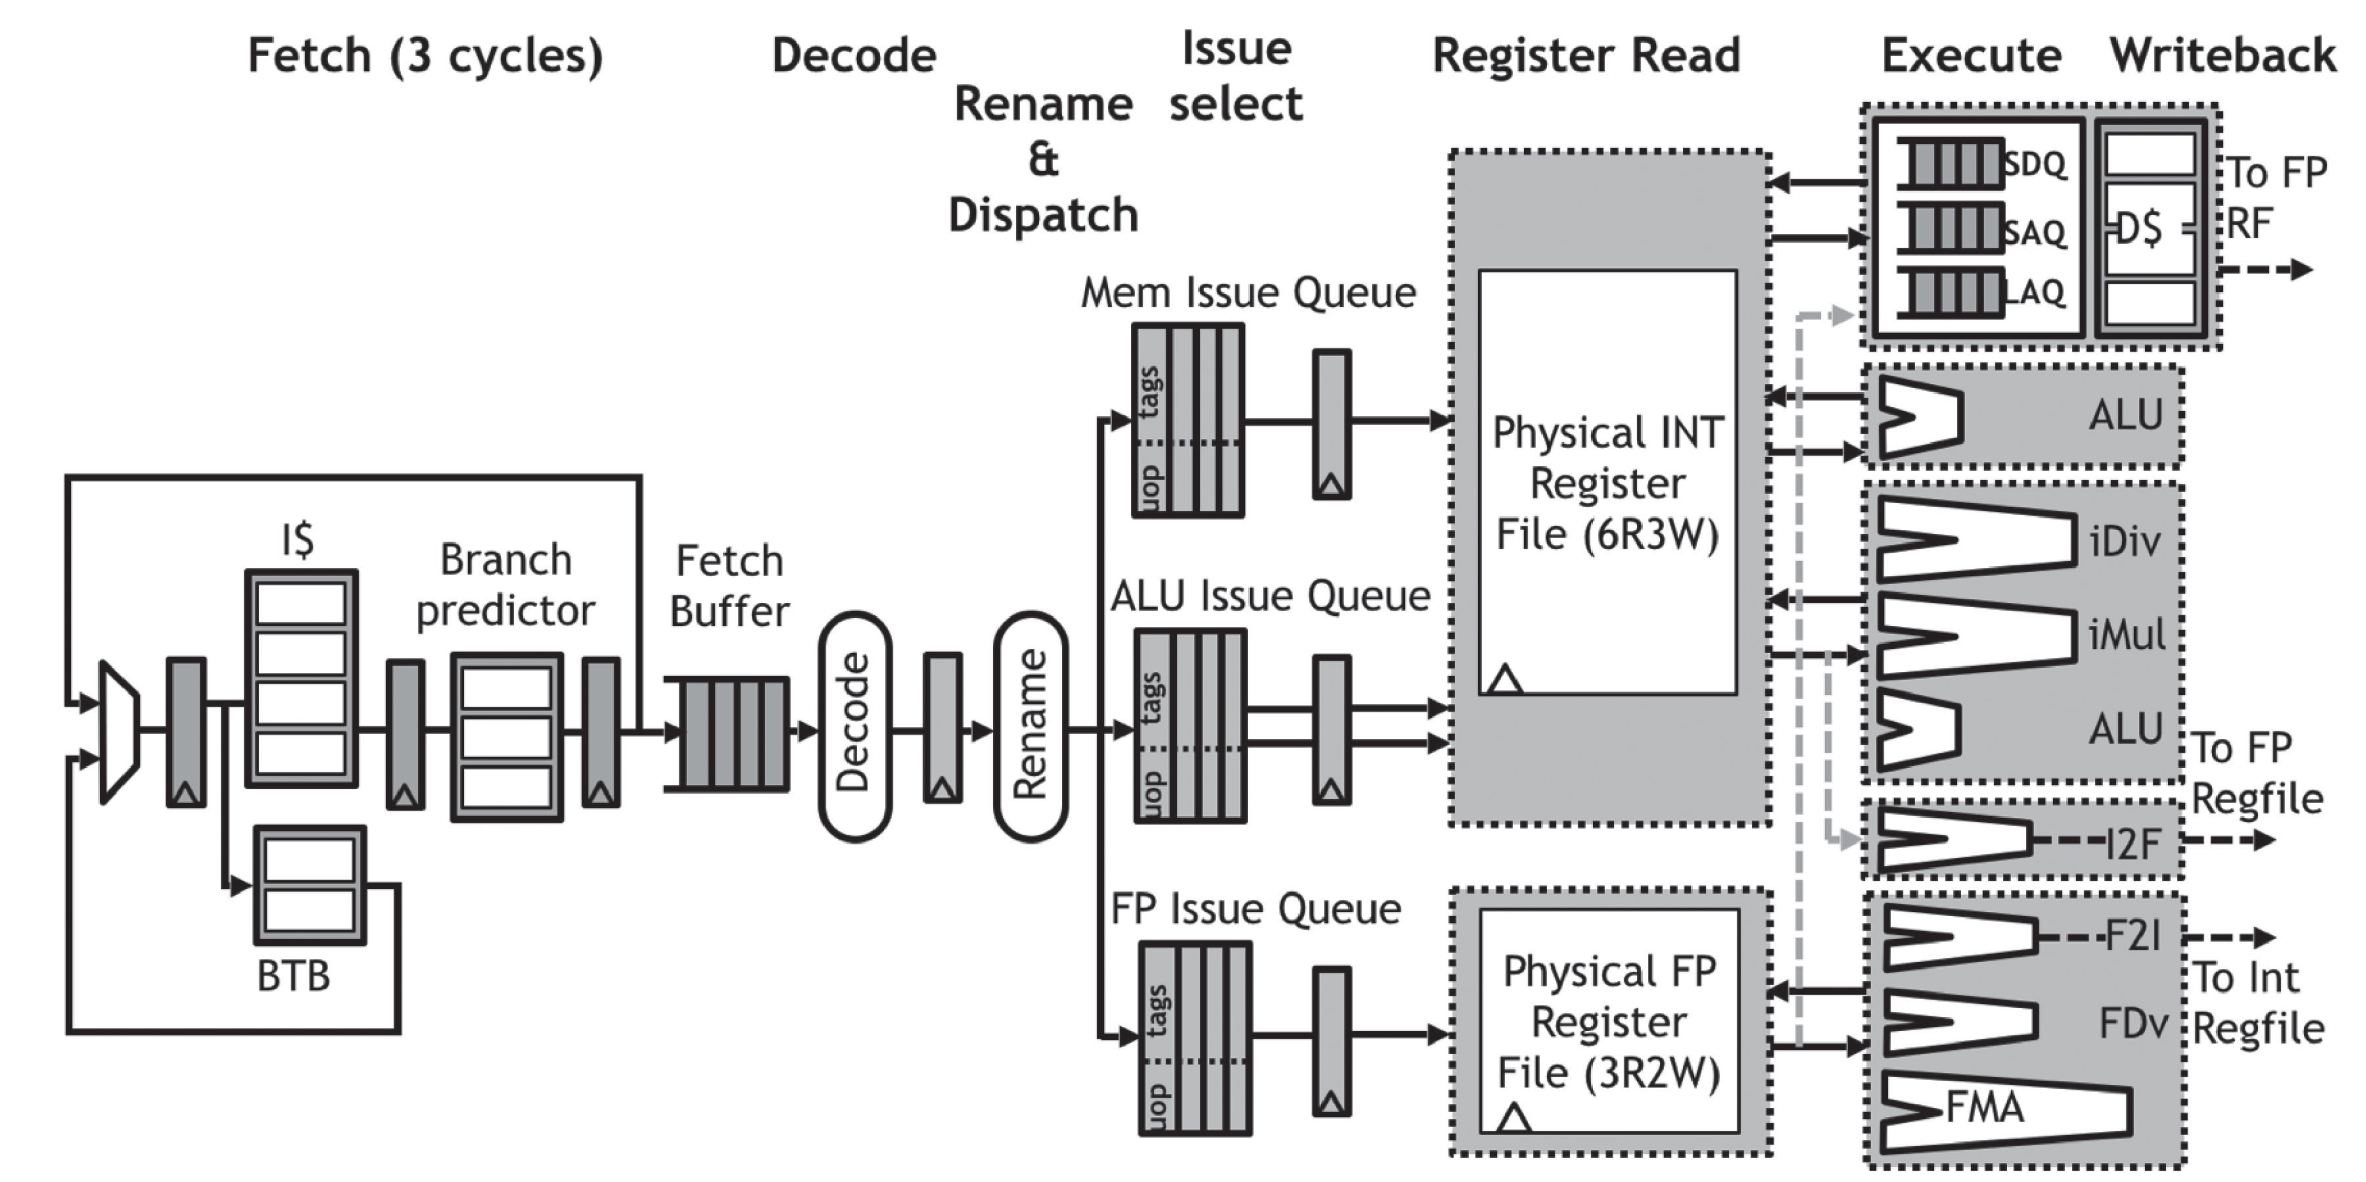
\includegraphics[width=15cm]{../ooo/broom-pipeline}
};
\end{tikzpicture}
\imagecredit{Figure from Celio et al., ``BROOM: An Open Source Out-Of-Order Processor With Resilient Low-Voltage  Operation in 28-nm CMOS''}
\end{frame}


\subsection{data flow limit}
\usetikzlibrary{shapes}

\begin{frame}[fragile,label=dfLimit]{data flow model and limits}
    \begin{tikzpicture}
        \tikzset{
            var/.style={draw,rectangle,fill=blue!30},
            op/.style={draw,ellipse,fill=yellow!40},
            node distance=4mm,
        }
        \begin{scope}[
                start chain=going below,
                every join/.style={thick,-Latex},
                every node/.style={on chain,op},
            ]
            \node[var] (sn1) at (0,1) {sum};
            \node[join] (s0)  {+};
            \node[join] (s1) {+};
            \node[join] (s2) {+};
            \node[join] (s3) {+};
        \end{scope}
        \node[var,right=2cm of s3] (sumFinal) {sum (final)};
        \draw[thick,-Latex] (s3) -- (sumFinal);
        \begin{scope}[
                start chain=going below,
                every node/.style={on chain,op},
            ]
            \node (l0) at (2,1) {load};
            \node (l1) {load};
            \node (l2) {load};
            \node (l3) {load};
        \end{scope}
        \begin{scope}[
                start chain=going below,
                every join/.style={thick,-Latex},
                every node/.style={on chain,op,join},
            ]
            \node[var] (a0) at (4,2.2) {A + i};
            \node (a1) {+ 1};
            \node (a2) {+ 1};
            \node (a3) {+ 1};
        \end{scope}
        \begin{visibleenv}<all:4>
        \node[op] (c1) at (7,1) {> A + N?};
        \draw[thick,-Latex] (a0) -- (c1);
        \node[op] (c3) at (7,-3) {> A + N?};
        \draw[thick,-Latex] (a3) -- (c3);
        \end{visibleenv}
        \begin{scope}[thick,-Latex]
            \foreach \x in {0,1,2,3} {
                \draw (a\x) -- (l\x) -- (s\x);
            }
        \end{scope}
        \begin{visibleenv}<all:1>
            \node[anchor=west] at ([xshift=1cm,yshift=-.5cm]a2.east) {
\begin{lstlisting}[language=C,style=small]
for (int i = 0; i < N; i += K) {
    sum += A[i];
    sum += A[i+1];
    ...
}
\end{lstlisting}
};
        \end{visibleenv}
        \begin{visibleenv}<all:2>
            \node[align=left,anchor=west] at (5, -1) {
                each yellow box = instruction\\
                arrows = dependences\\
                instructions only executed when dependencies ready
            };
        \end{visibleenv}
        \begin{visibleenv}<all:3>
            \node[draw,very thick,red,fit=(s0) (l1) (a2),label={east:three ops/cycle (\myemph{if} each one cycle)}] {};
        \end{visibleenv}
        \begin{visibleenv}<all:4>
            \node[draw,very thick,red,fit=(s0) (s3)] {};
            \node[align=left,anchor=west] at (5, -1) {
                can only do sums one at a time
            };
        \end{visibleenv}
    \end{tikzpicture}
\end{frame}



    % FIXME: remove or explain free list
    % FIXME: possibly use or mention two register files instead of mappings?

\subsection{multiple accumulator transformation}
\usetikzlibrary{chains,fit,shapes}

\begin{frame}{better data-flow}
    \begin{tikzpicture}
        \tikzset{
            var/.style={draw,rectangle,fill=blue!30},
            op/.style={draw,ellipse,fill=yellow!40},
            node distance=5mm,
        }
        \begin{scope}[
                start chain=going below,
                every join/.style={thick,-Latex},
                every node/.style={on chain,op},
            ]
            \node[var] (sn1) at (0,1) {sum1};
            \node[join] (s0)  {+};
            \node[join] (s1) {+};
            \node[join] (s2) {+};
        \end{scope}

        \begin{scope}[
                start chain=going below,
                every join/.style={thick,-Latex},
                every node/.style={on chain,op},
            ]
            \node[var] (tn1) at (10,1) {sum2};
            \node[join] (t0) {+};
            \node[join] (t1) {+};
            \node[join] (t2) {+};
        \end{scope}
        \begin{scope}[
                start chain=going below,
                every node/.style={on chain,op},
            ]
            \node (l0) at (2,1) {load};
            \node (l1) {load};
            \node (l2) {load};
        \end{scope}
        \begin{scope}[
                start chain=going below,
                every node/.style={on chain,op},
            ]
            \node (m0) at (8,1) {load};
            \node (m1) {load};
            \node (m2) {load};
        \end{scope}
        \begin{scope}[
                start chain=going below,
                every join/.style={thick,-Latex},
                every node/.style={on chain,op,join},
            ]
            \node[var] (a0) at (4,2.2) {A + i};
            \node (a1) {+ 2};
            \node (a2) {+ 2};
        \end{scope}
        \begin{scope}[
                start chain=going below,
                every join/.style={thick,-Latex},
                every node/.style={on chain,op,join},
            ]
            \node[var] (b0) at (6,2.2) {A + i + 1};
            \node (b1) {+ 2};
            \node (b2) {+ 2};
        \end{scope}
        \node[op] (combine) at (5, -4) {+};
        \node[below=.2cm of combine,var] (final) {sum (final)};
        \begin{scope}[thick,-Latex]
            \foreach \x in {0,1,2} {
                \draw (a\x) -- (l\x) -- (s\x);
                \draw (b\x) -- (m\x) -- (t\x);
            }
            \draw (s2) -- (combine);
            \draw (t2) -- (combine);
            \draw (combine) -- (final);
        \end{scope}
        \begin{visibleenv}<2>
            \node[draw,red, ultra thick,fit=(a2) (s0) (b2) (t0),label={[red!70!black,font=\bfseries,align=center]south: 6 ops/time \\ two sum adds/time}] {};
        \end{visibleenv}
        \begin{visibleenv}<3>
            \node[draw,red, ultra thick,fit=(s0) (s2)] {};
            \node[draw,red, ultra thick,fit=(t0) (t2)] {};
            \node[draw,red, ultra thick,fit=(combine),label={[red!70!black,font=\bfseries,align=center]north:4 adds of time --- 7 adds}] {};
        \end{visibleenv}
    \end{tikzpicture}
\end{frame}

